%%%%%%%%%%%%%%%%%%%%%%%%%%%%%%%%%%%%%%%%%%%%%%%%%%%%%%%%%%%%%%%%%%%%%%%%%%%%%%%%%%%%%%%%%%%%%%%%%%%%
%	chap02 (データの整理)
%===================================================================================================
%	AUTHOR	H. NAKAJIMA
%	DATE	2025/01
%===================================================================================================
%	EDIT HISTORY
%	DATE		NAME			OVERVIEW
%---------------------------------------------------------------------------------------------------
%	2025/01		H. NAKAJIMA		Create new
%%%%%%%%%%%%%%%%%%%%%%%%%%%%%%%%%%%%%%%%%%%%%%%%%%%%%%%%%%%%%%%%%%%%%%%%%%%%%%%%%%%%%%%%%%%%%%%%%%%%

{
	\centering
	{\textbf{第 2 章 \indent データの整理}} \\
}

{\textbf{\S 2.1 \indent 1 次元のデータ}}
\basic
\begin{qenumerate}
	\item{
		累積度数分布表は以下のようになる.
		\begin{table}[H]
			\centering
			\begin{tabular}{c|c|c} \hline
				階級値 (cm) & 累積度数 & 累積相対度数 \\ \hline
				164 &  5 & 0.125 \\
				168 & 13 & 0.325 \\
				172 & 25 & 0.625 \\
				176 & 31 & 0.775 \\
				180 & 36 & 0.900 \\
				184 & 40 & 1.000 \\ \hline
			\end{tabular}
		\end{table}
	}
	\item{
		ヒストグラムと度数折れ線は以下のようになる.
		\begin{figure}[H]
			\centering
			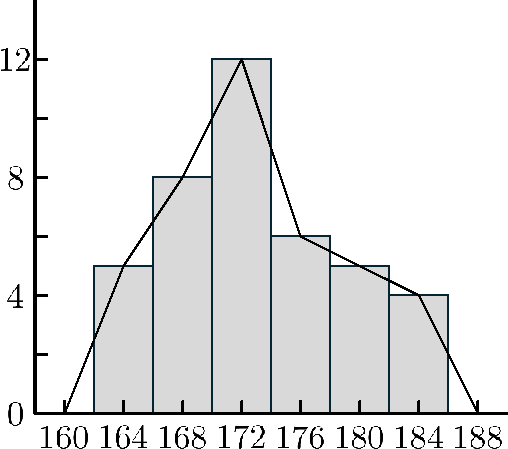
\includegraphics[scale = 0.5]{./figure/73.pdf}
		\end{figure}
	}
	\item{
		求める平均 $\overline{x}$ は
		\begin{align}
			\overline{x} &= \frac{5\cdot 164 \! + \! 8 \! \cdot \! 168 \! + \! 12 \! \cdot \! 172 \! + \! 6 \! \cdot \! 176 \! + \! 5 \! \cdot \! 180 \! + \! 4 \! \cdot \! 184}{40} \\
				&= \red{173}.
		\end{align}
	}
	\item{
		変換後のデータは
		\begin{align}
			u: \red{-12}, \quad \red{11}, \quad \red{-4}, \quad \red{15}, \quad \red{18}, \quad \red{-18}, \quad \red{16}
		\end{align}
		である.
		またデータの平均は, $\overline{u} = \dfrac{\overline{x} - 30}{0.01}$ より
		\begin{align}
			\overline{x} &= 0.01\overline{u} + 30 \\
				&= 0.01\cdot\frac{-12 \! + \! 11 \! + \! (-4) \! + \! 15 \! + \! 18 \! + \! (-18) \! + \! 16}{7} + 30 \\
				&\simeq 0.01\cdot 3.7 + 30 \\
				&\simeq \red{30.04}. 
		\end{align}
	}
	\item{
		\begin{enumerate}
			\item{
				平均値 $\overline{x}$ は
				\begin{align}
					\overline{x} = \frac{1 + 1 + 2 + 3 + 4 + 5 + 5 + 7 + 9 + 10}{10} = \red{4.7}.
				\end{align}
				データ数が偶数だから, 中央値は
				\begin{align}
					\frac{4 + 5}{2} = \red{4.5}.
				\end{align}
			}
			\item{
				平均値 $\overline{x}$ は
				\begin{align}
					\overline{x} = \frac{1 + 1 + 2 + 3 + 4 + 5 + 6 + 7 + 9 + 10 + 18}{11} = \red{6}.
				\end{align}
				データ数が奇数だから, 中央値は\red{5}.
			}
		\end{enumerate}
	}
	\item{
		度数が一番大きい階級は 60--65 だから, 最頻値は
		\begin{align}
			\frac{60 + 65}{2} = \red{62.5}.
		\end{align}
		データ数が 45 だから, 中央値は順に並んだデータの 23 番目のデータである.
		以下の累積度数分布表において, 累積度数が 23 になる階級は \red{55--60}.
		\begin{table}[H]
			\centering
			\begin{tabular}{c|c|c} \hline
				階級 & 度数 & 累積度数 \\ \hline
				40--45 &  2 &  2 \\
				45--50 &  4 &  6 \\
				50--55 & 12 & 18 \\
				\textbf{55--60} &  9 & \textbf{27} \\
				60--65 & 13 & 40 \\
				65--70 &  2 & 42 \\
				70--75 &  0 & 42 \\
				75--80 &  3 & 45 \\ \hline
			\end{tabular}
		\end{table}
	}
	\item{
		得点の最大値は 8, 最小値は 2 であるから, 範囲は $8 - 2 = \red{6}$.
		得点の平均 $\overline{x}$ は
		\begin{align}
			\overline{x} = \frac{4 + 6 + 2 + 8 + 3 + 6 + 5 + 3 + 6 + 7 + 5 + 8}{12} = \red{5.25}.
		\end{align}
		得点の分散 $v_{x}$ は
		\begin{align}
			v_{x} = \frac{(4 - 5.25)^{2} + \cdots + (8 - 5.25)^{2}}{12} \simeq 3.5208
		\end{align}
		であるから, 標準偏差 $s_{x}$ は
		\begin{align}
			s_{x} = \sqrt{v_{x}} = \sqrt{3.5208} = \red{1.876}.
		\end{align}
	}
	\item{
		気温の平均 $\overline{x}$ は
		\begin{align}
			\overline{x} &= \frac{19.6 + \cdots + 19.1}{10} = \red{20.65}.
		\end{align}
		気温の分散 $v_{x}$ は
		\begin{align}
			v_{x} = \frac{(19.6 - 20.65)^{2} + (19.1 - 20.65)^{2}}{10} = 7.8525
		\end{align}
		であるから, 標準偏差 $s_{x}$ は
		\begin{align}
			s_{x} = \sqrt{v_{x}} = \sqrt{7.8525} \simeq \red{2.802}.
		\end{align}
	}
	\item{
		女子学生の身長の平均 $\overline{x}$ は
		\begin{align}
			\overline{x} = \frac{4\cdot 146 + \cdots 2\cdot 174}{100} = \red{159.36}.
		\end{align}
		女子学生の身長の分散 $v_{x}$ は
		\begin{align}
			v_{x} = \frac{4\cdot (146 - 159.36)^{2} + 2\cdot (174 - 159.36)^{2}}{100} = 37.1904
		\end{align}
		であるから, 分散 $s_{x}$ は
		\begin{align}
			s_{x} = \sqrt{v_{x}} = \sqrt{37.1904} \simeq \red{6.098}.
		\end{align}
	}
\end{qenumerate}